\documentclass[11pt, a4paper]{article} 
\usepackage{booktabs}
\usepackage{comment} 
\usepackage[utf8]{inputenc}
\usepackage[T1, T2A]{fontenc} 
\usepackage{graphicx}
\usepackage{float}
\usepackage{multirow}
\usepackage{amsmath, amsfonts,amsthm} 
\usepackage{amsthm}
\usepackage{mathtools}
\usepackage{blindtext} 
\usepackage{geometry}
\usepackage{graphicx}
\usepackage{amssymb}
\usepackage{tikz-cd}
\usepackage{lscape}
\usepackage{hyperref}
\usepackage{XCharter}
\usepackage{dsfont}
\usepackage[labelfont=bf]{caption}
\usepackage{caption}
\usepackage{subcaption}
\usepackage{pbox}
\usepackage{tikz}
\usepackage{svg}

\setlength{\parindent}{15pt} 

\title{\vspace{-2cm}Landau pole in the Standard Model and the asymptotic safety}
\title{\vspace{-2cm}Landau pole in the Standard Model and the asymptotic safety}
\author{{Wojciech Śmiałek}\\
\\
{\textit{Supervisor}} \\
{Jan Kwapisz Ph.D.}}
{Jan Kwapisz Ph.D.}}
\date{}
\newcommand{\jhk}[1]{{\color{red}#1}}
\newcommand{\jhkbf}[1]{\textbf{\color{red} [#1]}}
\newcommand{\ws}[1]{{\color{cyan}#1}}
\newcommand{\wsbf}[1]{\textbf{\color{cyan} [#1]}}

\newcommand{\jhk}[1]{{\color{red}#1}}
\newcommand{\jhkbf}[1]{\textbf{\color{red} [#1]}}
\newcommand{\ws}[1]{{\color{cyan}#1}}
\newcommand{\wsbf}[1]{\textbf{\color{cyan} [#1]}}


\begin{document}
\maketitle

\section{Introduction}
\jhkbf{Tak zaznaczam komentarze}
\jhk{A tak poprawki}
\jhkbf{Użyj szablonu, link poniżej: }
%https://mimuw.edu.pl/wzor-pracy-magisterskiej-i-licencjackiej

\section{Introduction}
\jhkbf{Tak zaznaczam komentarze}
\jhk{A tak poprawki}
\jhkbf{Użyj szablonu, link poniżej: }
%https://mimuw.edu.pl/wzor-pracy-magisterskiej-i-licencjackiej


\section{Standard model ...}
\subsection{Renormalization in the Standard Model}
The Standard Model of particle physics is a unified description of all quantum fields observed in subatomic physics.  \jhkbf{What about gravity?}
\subsection{Renormalization in the Standard Model}
The Standard Model of particle physics is a unified description of all quantum fields observed in subatomic physics.  \jhkbf{What about gravity?}
It strives to predict all the phenomena observed at microscopic scales while maintaining theoretical
self-consistency and certain mathematical aesthetics. The predictive power of the Standard Model, with its most
self-consistency and certain mathematical aesthetics. The predictive power of the Standard Model, with its most
famous examples like precision tests of electron anomalous magnetic moment or the discovery of Higgs boson,
makes it ungrounded to postulate a fundamental physical theory that would not reduce to SM in the suitable limit, at least
as an effective field theory.
Standard Model, however, certainly is not a complete theory of physical reality. It does not include a description
of gravity and above the Planck scale $E_p \approx 10^{19} \ \text{GeV}$, due to quantum effects of gravity,
predictions of both the SM and Einstein's theory of gravity are not expected to apply.
One should then not be surprised if above $E_p$ Standard Model exhibits certain inconsistencies.
Effective behaviour of the gauge interactions in Standard Model at different energy scales is governed by the renormalization group equations (RGEs) of three parameters: $U(1)$ gauge coupling $g_1$, $U(2)$ gauge coupling $g_2$ and $U(3)$ gauge coupling $g_3$.
\begin{gather}
   \beta_{g_1} = \frac{41}{96\pi^2} g_1^3 + \mathcal{O}(g_1^5) \\% = b^{\text{SM}} g_1^3
    \beta_{g_2} = - \frac{19}{96\pi^2} g_2^3  + \mathcal{O}(g_2^5)\\
    \beta_{g_3} = - \frac{7}{16\pi^2} g_3^3 + \mathcal{O}(g_3^5) \\
    % \beta_{h} = \frac{1}{16 \pi^2} \left[ \frac{9}{2} h^3 -8g_3^2 h- \frac{9}{4} g_2^2 - \frac{17}{12} g_1^2 h \right]\\
    % \beta_{\lambda} =  \frac{1}{16 \pi^2} \left[ 24 \lambda^2 + 12 \lambda h^2 -9\lambda (g_2^2 + \frac{1}{3} g_1^2) - 6 h^4 + \frac{9}{8} g_2^4 + \frac{3}{8} g_1^4 +\frac{3}{4} g_2^2 g_1^2 \right]
\end{gather}
Where $\beta_{x_j} = \mu \partial_\mu x_j$ are the Callan - Symanzik beta functions and $\mu$ is the renormalization scale, defined as the ratio between the characteristic energy $\Lambda$ of a given process and a reference scale $k_0$ at which the value of coupling is fixed by the observation.
The higgs mass $m_h$, scalar self-interaction coupling $\lambda$ and three matrices of Yukawa interaction between the fermions and higgs field constitute all the remaining scale dependent couplings of the SM \textcolor{red}{(?)}.
The differential equation of the general form $\mu \partial_\mu g = b g^3$ can be integrated and if the value of coupling at scale $k_0$ is fixed to be the measured value $g_{\text{obs}}$, then the predicted $g(\mu)$ at different energy scales is given by
One should then not be surprised if above $E_p$ Standard Model exhibits certain inconsistencies.
Effective behaviour of the gauge interactions in Standard Model at different energy scales is governed by the renormalization group equations (RGEs) of three parameters: $U(1)$ gauge coupling $g_1$, $U(2)$ gauge coupling $g_2$ and $U(3)$ gauge coupling $g_3$.
\begin{gather}
   \beta_{g_1} = \frac{41}{96\pi^2} g_1^3 + \mathcal{O}(g_1^5) \\% = b^{\text{SM}} g_1^3
    \beta_{g_2} = - \frac{19}{96\pi^2} g_2^3  + \mathcal{O}(g_2^5)\\
    \beta_{g_3} = - \frac{7}{16\pi^2} g_3^3 + \mathcal{O}(g_3^5) \\
    % \beta_{h} = \frac{1}{16 \pi^2} \left[ \frac{9}{2} h^3 -8g_3^2 h- \frac{9}{4} g_2^2 - \frac{17}{12} g_1^2 h \right]\\
    % \beta_{\lambda} =  \frac{1}{16 \pi^2} \left[ 24 \lambda^2 + 12 \lambda h^2 -9\lambda (g_2^2 + \frac{1}{3} g_1^2) - 6 h^4 + \frac{9}{8} g_2^4 + \frac{3}{8} g_1^4 +\frac{3}{4} g_2^2 g_1^2 \right]
\end{gather}
Where $\beta_{x_j} = \mu \partial_\mu x_j$ are the Callan - Symanzik beta functions and $\mu$ is the renormalization scale, defined as the ratio between the characteristic energy $\Lambda$ of a given process and a reference scale $k_0$ at which the value of coupling is fixed by the observation.
The higgs mass $m_h$, scalar self-interaction coupling $\lambda$ and three matrices of Yukawa interaction between the fermions and higgs field constitute all the remaining scale dependent couplings of the SM \textcolor{red}{(?)}.
The differential equation of the general form $\mu \partial_\mu g = b g^3$ can be integrated and if the value of coupling at scale $k_0$ is fixed to be the measured value $g_{\text{obs}}$, then the predicted $g(\mu)$ at different energy scales is given by
\begin{equation}
    g(\mu) = \frac{g_{\text{obs}}}{\sqrt{1-2g_{\text{obs}}^2 b \log{\mu}}}
    g(\mu) = \frac{g_{\text{obs}}}{\sqrt{1-2g_{\text{obs}}^2 b \log{\mu}}}
\end{equation}
The negativity of $\beta_{g_2}$ and $\beta{g_3}$ ensures that for any positive observed value of these couplings, in the limit $\mu \rightarrow \infty$ they tend to zero. This behaviour is called the asymptotic freedom.
The beta function of the abelian gauge coupling $g_1$ however is positive and
there exist a finite $\mu= \left(2 g_{\text{obs}}^2 \ \beta_{g}^{(3)} \right)^{-1} $, at which the expression becomes singular.
This is known as the Landau pole or the quantum triviality problem and
it remains as one of the big issues of the SM.
% is the quantum triviality problem for the electroweak $U(1)$ gauge coupling and
% the scalar higgs boson quartic coupling.
% In the pure electroweak theory, one loop $\beta$-function of the abelian gauge coupling $g$ is: \cite{higgs mass}
% \begin{equation}
%     \beta_{g}^{\text{SM}} = \beta_{g}^{(3)} g^3 = \frac{41}{6} \frac{g_1^3}{16 \pi^2},
% \end{equation}
% % \jhkbf{What is Y?}

% - rge can be integrated
% - g(mu)
% - widać że asymptotycznie do zera dla ujemnych beta - nazywamy as. freedom i że biegun w skończonej skali gdy dodatnia beta - problem w modelu st. landau pole also called the quantum triviality problem

% Wywalić z tym bare value

% If one postulates that the bare value of a coupling, i.e. $g_{\infty}=\lim_{\mu\rightarrow\infty} g(\mu)$ is the 'true' physical value and it has to be finite,
% then the value observed in the low energy limit $g_{\text{obs}}$ implied by the SM will be given by
% \begin{equation}
%     g_{\text{obs}} = \lim_{\mu\rightarrow\infty} \frac{g_{\infty}}{\sqrt{1+2g_{\infty}^2\beta_g^{(3)}\log{\mu}}}
% \end{equation}
% This implies a trivial theory with $g=0$ in the low energy limit for any finite value of bare coupling, which clearly contradicts the observations.
% Conversely, if we take the measured value $g_{\text{obs}}$ as an input, the predicted value of gauge coupling at different energy scales is
% \begin{equation}
%     g(\mu) = \frac{g_{\text{obs}}}{\sqrt{1-2g_{\text{obs}}^2 \beta_g^{(3)}\log{\mu}}}
% \end{equation}
% and the $g(\mu)$ diverges at a scale $\mu = \left(2 g_{\text{obs}}^2 \ \beta_{g}^{(3)} \right)^{-1} $.
% This is known as the Landau pole.
% Conversely, one could postulate that the bare value of a coupling, i.e. $g_{\infty}=\lim_{\mu\rightarrow\infty} g(\mu)$ is the 'true' physical value and it has to be finite. 
% Then, the value observed in the low energy limit $g_{\text{obs}}$ should be given by
% \begin{equation}
%     g_{\text{obs}} = \lim_{\mu\rightarrow\infty} \frac{g_{\infty}}{\sqrt{1+2g_{\infty}^2\beta_g^{(3)}\log{\mu}}}
% \end{equation}
% This implies a trivial theory with $g=0$ in the low energy limit for any finite value of $g_{\infty}$, which clearly contradicts the observations.
% taking any arbitrarily high value of the bare coupling, the only possible value of $g_{\text{obs}}$ should be 0, making
% the theory trivial, i.e. non-interacting. \jhkbf{Dlaczego? Bo co inaczej? Co to jest bare coupling?}
The negativity of $\beta_{g_2}$ and $\beta{g_3}$ ensures that for any positive observed value of these couplings, in the limit $\mu \rightarrow \infty$ they tend to zero. This behaviour is called the asymptotic freedom.
The beta function of the abelian gauge coupling $g_1$ however is positive and
there exist a finite $\mu= \left(2 g_{\text{obs}}^2 \ \beta_{g}^{(3)} \right)^{-1} $, at which the expression becomes singular.
This is known as the Landau pole or the quantum triviality problem and
it remains as one of the big issues of the SM.
% is the quantum triviality problem for the electroweak $U(1)$ gauge coupling and
% the scalar higgs boson quartic coupling.
% In the pure electroweak theory, one loop $\beta$-function of the abelian gauge coupling $g$ is: \cite{higgs mass}
% \begin{equation}
%     \beta_{g}^{\text{SM}} = \beta_{g}^{(3)} g^3 = \frac{41}{6} \frac{g_1^3}{16 \pi^2},
% \end{equation}
% % \jhkbf{What is Y?}

% - rge can be integrated
% - g(mu)
% - widać że asymptotycznie do zera dla ujemnych beta - nazywamy as. freedom i że biegun w skończonej skali gdy dodatnia beta - problem w modelu st. landau pole also called the quantum triviality problem

% Wywalić z tym bare value

% If one postulates that the bare value of a coupling, i.e. $g_{\infty}=\lim_{\mu\rightarrow\infty} g(\mu)$ is the 'true' physical value and it has to be finite,
% then the value observed in the low energy limit $g_{\text{obs}}$ implied by the SM will be given by
% \begin{equation}
%     g_{\text{obs}} = \lim_{\mu\rightarrow\infty} \frac{g_{\infty}}{\sqrt{1+2g_{\infty}^2\beta_g^{(3)}\log{\mu}}}
% \end{equation}
% This implies a trivial theory with $g=0$ in the low energy limit for any finite value of bare coupling, which clearly contradicts the observations.
% Conversely, if we take the measured value $g_{\text{obs}}$ as an input, the predicted value of gauge coupling at different energy scales is
% \begin{equation}
%     g(\mu) = \frac{g_{\text{obs}}}{\sqrt{1-2g_{\text{obs}}^2 \beta_g^{(3)}\log{\mu}}}
% \end{equation}
% and the $g(\mu)$ diverges at a scale $\mu = \left(2 g_{\text{obs}}^2 \ \beta_{g}^{(3)} \right)^{-1} $.
% This is known as the Landau pole.
% Conversely, one could postulate that the bare value of a coupling, i.e. $g_{\infty}=\lim_{\mu\rightarrow\infty} g(\mu)$ is the 'true' physical value and it has to be finite. 
% Then, the value observed in the low energy limit $g_{\text{obs}}$ should be given by
% \begin{equation}
%     g_{\text{obs}} = \lim_{\mu\rightarrow\infty} \frac{g_{\infty}}{\sqrt{1+2g_{\infty}^2\beta_g^{(3)}\log{\mu}}}
% \end{equation}
% This implies a trivial theory with $g=0$ in the low energy limit for any finite value of $g_{\infty}$, which clearly contradicts the observations.
% taking any arbitrarily high value of the bare coupling, the only possible value of $g_{\text{obs}}$ should be 0, making
% the theory trivial, i.e. non-interacting. \jhkbf{Dlaczego? Bo co inaczej? Co to jest bare coupling?}
\begin{figure}[H]
    \includegraphics[width=1\textwidth]{./figures/plotr.jpg}
    \caption{Running of the abelian gauge parameter $\alpha_{Y} = \frac{g_1^2}{4\pi}$ in the Standard Model. Observed value $\alpha_{Y\text{obs}}$ is taken from \cite{pdg}. 
    Landau Pole marked at $\mu \approx 10^{42.5}$. \jhkbf{Większe podpisy.}}
    \caption{Running of the abelian gauge parameter $\alpha_{Y} = \frac{g_1^2}{4\pi}$ in the Standard Model. Observed value $\alpha_{Y\text{obs}}$ is taken from \cite{pdg}. 
    Landau Pole marked at $\mu \approx 10^{42.5}$. \jhkbf{Większe podpisy.}}
    \label{boxes}
\end{figure}
% For theories involving massive particles, dimensionless renormalization scale $\mu$ can be defined as the ratio between the characteristic energy $\Lambda$ of a given process and a mass of involved particles. 
Taking an electron mass as a reference scale of electroweak theory, the location of abelian coupling Landau pole 
% \jhkbf{Musisz dać definicję.} 
will be of order $\Lambda \sim 10^{48} \ \text{eV}$, which is well above the Planck scale.
Similarly, quartic self-interaction $\lambda$ of higgs field theoretically may exhibit a Landau pole at a finite momentum scale.
\end{figure}
% For theories involving massive particles, dimensionless renormalization scale $\mu$ can be defined as the ratio between the characteristic energy $\Lambda$ of a given process and a mass of involved particles. 
Taking an electron mass as a reference scale of electroweak theory, the location of abelian coupling Landau pole 
% \jhkbf{Musisz dać definicję.} 
will be of order $\Lambda \sim 10^{48} \ \text{eV}$, which is well above the Planck scale.
Similarly, quartic self-interaction $\lambda$ of higgs field theoretically may exhibit a Landau pole at a finite momentum scale.
Existence of both poles remains an open question, but a theory containing any such singularity cannot be fundamental.
One solution to this problem could be a grand unified theory (GUT), which proposes a larger symmetry group, spontaneously broken
to the known $SU(3)\times SU(2) \times U(1)$ of standard model at around the scale where running values of electroweak and strong couplings
coincide. This scale is predicted to be below Planck energy [ref]. Above the GUT scale, the theory could introduce
coincide. This scale is predicted to be below Planck energy [ref]. Above the GUT scale, the theory could introduce
a running of unified coupling that does not exhibit a triviality issue.
The existence of grand unification, however has not been yet confirmed in any way, while the experimental bounds on the proton lifetime
heavily constraints or even rules out many of the GUTs[ref]. This constrasts sharply with the other potential completion of the SM,
which is quantum gravity. Although no quantum theory of gravity has been widely accepted, the existence of gravity and
the quantum nature of physical reality most certainly are. Should quantum gravitational solution to the triviality issues of SM exist,
it would provide an argument for consistency between the particular theory of quantum gravity and the SM, as well as eliminate one of the arguments for the need of GUT.
\subsection{Running of gauge coupling in the effective field theory of quantum gravity}
it would provide an argument for consistency between the particular theory of quantum gravity and the SM, as well as eliminate one of the arguments for the need of GUT.
\subsection{Running of gauge coupling in the effective field theory of quantum gravity}
The straightforward approach to quantum gravity - a metric fluctuation quantum field governed by Einstein - Hilbert action
is known to be non-renormalizable by the perturbative methods.\cite{book}. However, for energy scales small
compared to Planck energy, the infinite number of divergent terms in the lagrangian affects predictions in a negligible way and can be effectively ignored.
is known to be non-renormalizable by the perturbative methods.\cite{book}. However, for energy scales small
compared to Planck energy, the infinite number of divergent terms in the lagrangian affects predictions in a negligible way and can be effectively ignored.
In this framework, called the effective field theory of gravity (EFT), there has been a number of works investigating
the gravitational contribution to the running of gauge couplings. The predictions of EFT does not apply above
the Planck scale, but an assessment of the quantitative nature of gravitational corrections can still give valuable information.
the Planck scale, but an assessment of the quantitative nature of gravitational corrections can still give valuable information.
Since gravitons carry no gauge charge, the contribution to beta function of gauge coupling from SM particles and gravitons are separate
and in the one-loop approximation takes the general form
\begin{equation}
    \beta_g(k) = \alpha \cdot G k^2 g + \gamma \cdot g^3 = \alpha \cdot G k^2 g + \beta_{g}^{\text{SM}}
    \beta_g(k) = \alpha \cdot G k^2 g + \gamma \cdot g^3 = \alpha \cdot G k^2 g + \beta_{g}^{\text{SM}}
    \label{betawilczek}
\end{equation}
The solution to the quantum triviality problem therefore depends on the value of $\alpha$.
For any positive value of $\alpha$, value of gauge coupling will contain a pole for some finite momentum scale.
Assuming $\alpha < 0$ and integrating the equation (\ref{betawilczek}), we find the equation determining the critical value $\alpha_{\text{crit}}$, below which the gauge coupling will be asymptotically free and above which it will contain the Landau pole
\begin{equation}
\operatorname{Ei}\left[\alpha_{\text{crit}} \left( \frac{k_0}{M_p} \right)^2 \right]
    = - \frac{e^{\alpha_{\text{crit}} \left( \frac{k_0}{M_p} \right)^2}}{b \ g^2(k_0)}% \approx  - \frac{1}{b \ g^2(k_0)}
\end{equation}
Where $\operatorname{Ei}(x)$ is the exponential integral function and $g(k_0)$ is the value of coupling observed at the momentum scale $k_0$. With the assumptions $b g^2(k_0) \ll 1$ and $k_0 \ll M_p$ the solution to this equation is approximately
% Inserting the observed value of abelian coupling of standard model for $g(k_0)$ and the electron mass for $k_0$, we obtain
\begin{equation}
    \alpha_{\text{crit}} \approx \left( \frac{M_p}{k_0} \right)^2 \operatorname{exp}{\left( - \frac{1}{b g^2(k_0)} \right)}
\end{equation}
Which for any realistic value of $g(k_0)$ results in an extremely tiny $\alpha_{\text{crit}}$, despite the large factor $M_p^2/k_0^2$.
This means that in practice determining the sign of gravitational contribution $\alpha$ is enough to conclude about the asymptotic freedom or the existence of a Landau pole.


The study of gravitational corrections to the running of abelian gauge coupling in the effective field theory of quantum gravity has generally produced contradicting results about the existence and sign of $\alpha$.
Initially, calculations in the cutoff scheme were performed by Wilczek and Robinson \cite{wilczek} and indicated
$\alpha = - \frac{3}{\pi} $, suggesting a solution to the triviality problem.
However, later work by Pietrykowski \cite{pietrykowski} argued, that a result obtained by Wilczek and Robinson is specific to the choice of graviton gauge fixing.
Using the same type of gauge fixing, Pietrykowski has reproduced the result of Wilczek and Robinson and confirmed that it does not depend on the value of gauge fixing parameter, but when using a different class of gauge fixing terms, he found the gravitational contribution to be absent.
In \cite{toms}, a Vilkovsky-DeWitt method was used and the calculations also indicated no gravitational contribution to $\beta_g$.
In \cite{absence}, calculations performed in both cutoff and dimensional regularization shemes indicated the absence of gravitational contribution.
Then, some later works again argued that the Wilczek's result was generally correct, for example the application of Loop Regularization method, which can appropriately treat the quadratic divergences and preserve non-abelian gauge symmetry,
indicated a non-vanishing contribution $\alpha = -\frac{1}{\pi} $ \cite{tang}.
The consensus has not yet been found and the question of the existence and value of $\alpha$ in the EFT is left open.
The solution to the quantum triviality problem therefore depends on the value of $\alpha$.
For any positive value of $\alpha$, value of gauge coupling will contain a pole for some finite momentum scale.
Assuming $\alpha < 0$ and integrating the equation (\ref{betawilczek}), we find the equation determining the critical value $\alpha_{\text{crit}}$, below which the gauge coupling will be asymptotically free and above which it will contain the Landau pole
\begin{equation}
\operatorname{Ei}\left[\alpha_{\text{crit}} \left( \frac{k_0}{M_p} \right)^2 \right]
    = - \frac{e^{\alpha_{\text{crit}} \left( \frac{k_0}{M_p} \right)^2}}{b \ g^2(k_0)}% \approx  - \frac{1}{b \ g^2(k_0)}
\end{equation}
Where $\operatorname{Ei}(x)$ is the exponential integral function and $g(k_0)$ is the value of coupling observed at the momentum scale $k_0$. With the assumptions $b g^2(k_0) \ll 1$ and $k_0 \ll M_p$ the solution to this equation is approximately
% Inserting the observed value of abelian coupling of standard model for $g(k_0)$ and the electron mass for $k_0$, we obtain
\begin{equation}
    \alpha_{\text{crit}} \approx \left( \frac{M_p}{k_0} \right)^2 \operatorname{exp}{\left( - \frac{1}{b g^2(k_0)} \right)}
\end{equation}
Which for any realistic value of $g(k_0)$ results in an extremely tiny $\alpha_{\text{crit}}$, despite the large factor $M_p^2/k_0^2$.
This means that in practice determining the sign of gravitational contribution $\alpha$ is enough to conclude about the asymptotic freedom or the existence of a Landau pole.


The study of gravitational corrections to the running of abelian gauge coupling in the effective field theory of quantum gravity has generally produced contradicting results about the existence and sign of $\alpha$.
Initially, calculations in the cutoff scheme were performed by Wilczek and Robinson \cite{wilczek} and indicated
$\alpha = - \frac{3}{\pi} $, suggesting a solution to the triviality problem.
However, later work by Pietrykowski \cite{pietrykowski} argued, that a result obtained by Wilczek and Robinson is specific to the choice of graviton gauge fixing.
Using the same type of gauge fixing, Pietrykowski has reproduced the result of Wilczek and Robinson and confirmed that it does not depend on the value of gauge fixing parameter, but when using a different class of gauge fixing terms, he found the gravitational contribution to be absent.
In \cite{toms}, a Vilkovsky-DeWitt method was used and the calculations also indicated no gravitational contribution to $\beta_g$.
In \cite{absence}, calculations performed in both cutoff and dimensional regularization shemes indicated the absence of gravitational contribution.
Then, some later works again argued that the Wilczek's result was generally correct, for example the application of Loop Regularization method, which can appropriately treat the quadratic divergences and preserve non-abelian gauge symmetry,
indicated a non-vanishing contribution $\alpha = -\frac{1}{\pi} $ \cite{tang}.
The consensus has not yet been found and the question of the existence and value of $\alpha$ in the EFT is left open.
The conceptual problem of EFT in this setting is the use of perturbative methods for scales approaching Planck energy.
Also, the use of some renormalization shemes for extracting beta functions is problematic, as e.g. dimensional regularization is insensitive to quadratic
divergences that are claimed to give contribution to $\beta_g$ \cite{absence}.
Adressing the problem properly would require the use of non-perturbative methods and mathematical tools that are more well-behaved.
A framework which we will discuss and conduct our own calculations in, is the quantum einstein gravity treated with functional renormalization group, also known as the asymptotic safety programme, which operates with the mathematical tools that are not ambiguous and
is conjectured to be valid also above the Planck scale \cite{qeg}.
Adressing the problem properly would require the use of non-perturbative methods and mathematical tools that are more well-behaved.
A framework which we will discuss and conduct our own calculations in, is the quantum einstein gravity treated with functional renormalization group, also known as the asymptotic safety programme, which operates with the mathematical tools that are not ambiguous and
is conjectured to be valid also above the Planck scale \cite{qeg}.

% (Segway into the asymptotic safety i że teraz nie effective tylko potentially uv complete)

% (I tutaj napisać jak AS to rozwiązało i przewidziało masę higgsa więc dobry trop i wogle)
% Wspomnieć że jeżeli biegun landaua zostanie, to nasz model musi być no najwyżej teorią efektywną
% I dopisać że do przewidzenia masy higgsa potrzeba żeby wkład od grawitacji do U(1) był ujemny, co my tutaj pokazujemy

% For the abelian gauge coupling $g$ with vanishing
% canonical dimension, the Ward-Takahashi identities imply a relation between the $\beta$-function of the coupling and the anomalous
% dimension $\eta_A$ of the gauge field. In the pure electroweak theory 
% Landau Pole
% Landau Pole for abelian hypercharge - figure
% + AS resolution of higgs triviality

\section{The Asymptotic safety approach to quantum gravity}
\subsection{The effective action}

% \jhkbf{Wyjaśnij te pojęcia dlaczego są ważne dla QFT i oznaczenia}
% The central object of the functional renormalization group is the effective average action. To construct it,
% for a theory including any number of scalar quantum fields denoted $\phi^a$,
% we begin with the definition of partition functional and the generating functional of connected Green's functions:
% \begin{gather}
%     Z[J] = \int \mathcal{D}\Phi \ e^{-S_E[\Phi] - \int dx j_a \phi^a} \\
%     W[J] = \log{Z[J]}
% \end{gather}
The central object of the functional renormalization group is the effective average action. To construct it,
for a theory including any number of scalar quantum fields denoted $\phi^a$,
we begin with the definition of a partition functional:
\begin{equation}
    Z[J] = \int \mathcal{D}\Phi \ e^{-S_E[\Phi] - \int d x j_a \phi^a}
    \label{zet}
\end{equation}
% To introduce it, let us start from the scalar field theory. The definition for other theories come as a straight-forward generalization.
% From now on, we will assume a Wick rotation
% and all scalar products should be understood as euclidean.
% The partition function and the generating functional of connected Green's functions reads
Where $J$, $\Phi$ denotes all currents and fields collectively and $S_E[\Phi]$ is a Wick-rotated action.
The Wick rotation in the static Minkowski space is an analytic continuation to the imaginary time coordinate, which acts as a mathematical trick, greatly simplifying calculations. Defining a Wick rotation in the general relativity is more subtle and a class of manifolds that admits it is restricted. For a more exhaustive discussion, see [ref].
From now on, the subscript $E$ will be skipped and any scalar products of four-vectors should be understood as euclidean, with the metric $g^{\mu\nu} = \delta^{\mu\nu}$.

The partition functional is the key object of study in the path integral formalism of quantum field theory.
It can be understood as the sum of all possible quantum field configurations weighted with exponent of their negative action.
Explicit evaluation of the values of $Z[J]$ is feasible only for $Z[0]$ in the non-interacting theory, however in practice one does not need to calculate specific values of $Z[J]$. The most useful property of the partition functional is the relation between its functional derivatives and the correlation functions:
\begin{equation}
G^{(n)}(x_1,\dots,x_n) =
\frac{\langle 0| \mathcal{T} \phi(x_1) \dots \phi(x_n) \hat{S} |0\rangle}{\langle 0 | \hat S |0\rangle} = 
(-1)^n \frac{1}{Z[0]}\left.\frac{\delta^n Z[J]}{\delta J(x_1) \dots \delta J(x_n)}\right|_{J=0}
\end{equation}
Given the correlation functions one can calculate via the LSZ reduction formula any $S$-matrix element and from there, any cross section of the scattering process.
$G^{(n)}$ receives contribution from all the disconnected Feynman diagrams apart from the vacuum bubbles, which exactly cancels with the normalization factor $Z[0]$.
% The general correlation functions can describe any processes such as experiments carried out in two laboratories far away or the aplitudes for ... however they can always be expressed in terms of the sums of all connected diagrams. This gives rise to the simple formula that relates the $Z[J]$ to the generating functional of the connected correlation functions:
The correlation functions in general describe the amplitudes for any possible transitions such as in independent experiments carried out in two laboratories far away. They are however always expressed in terms of the products of sums of connected diagrams. This gives rise to the formula relating $Z[J]$ and the generating functional $W[J]$ of the connected correlation functions $G_c^{(n)}$, which turns out to be a simple exponentiation:
\begin{gather}
    Z[J] = e^{W[J]}\\
    G_c^{(n)}(x_1,\dots,x_n) = (-1)^{n-1} \left.\frac{ \delta^n W[J]}{\delta J(x_1) \dots \delta J(x_n)}\right|_{J=0}
\end{gather}

% Here $G^{(n)}$ are the connected n-point correlation functions. In the functional derivative of $W[J]$, the normalization factor $Z[0]$, also interpreted as the sum of vacuum bubble diagrams or the vacuum energy density, cancels out and $W[J]$ directly acts as a generating functional of $G^{(n)}$.
% (...)
In principle, for a theory which interacts weakly and can be viewed as a small perturbation of the free theory, correlation functions should now be easily computed up to desired order of perturbation as a sum of relevant diagrams with values assigned by the Feynman rules, arising from the combinatorics of funtional derivative acting on the generating functional.
These diagrams can be classified in yet another useful way,
as the tree-level and loop diagrams.
(obrazek)
The values assigned to tree-level diagrams are simple products of theory's propagators and vertices and there is no ambiguity in evaluating them.
The problem appears, when one evaluates particular loop diagrams, which contain divergent integrals over momentum space, indicating that the amplitude receives contribution from arbitrarily high-momentum quantum fluctuations
This divergences has to be well-understood and treated carefully, being the key to retain physical meaning and the predictive power of interacting QFTs.
An important conceptual simplification of this problem comes from separating the tree-level and loop structure of diagrams, giving rise to the notion of effective action.
Using the sum of diagrams in which cutting no single internal line results in disconnected diagram, called the one particle irreducible diagrams, it is possible to construct what is called the exact vertices and propagators.
These corrected vertices and propagators take into account all the divergent loop integrals or equivalently all of the quantum fluctuations.
Then, a correlation functions could be constructed simply as the sum of tree-level diagrams, where propagators and vertices have been replaced by their exact counterparts.
(obrazek)
A generating functional of the exact vertices or the 1PI correlation functions would then be understood as the effective "quantum - corrected" action.
It can be shown that this functional, called the effective action and denoted as $\Gamma$ is the Legendre transform of $W[J]$:
\begin{equation}
    \Gamma[\Phi_c] = W[J_\Phi] - \int d^4 x {j_\phi}_a(x) \phi^a(x)
    \Gamma[\Phi_c] = W[J_\Phi] - \int d^4 x {j_\phi}_a(x) \phi^a(x)
\end{equation}
Where the two fields $\Phi_c$ and $J_\Phi$ are inverses of each other, defined as the solution to
\begin{equation}
    \Phi_c(x) = \langle \hat\Phi (x) \rangle_{J} = \frac{\delta W[J]}{\delta J(x)}
\end{equation}
The argument of the effective action is a vacuum expectation value of the quantum field and there is no functional integral to be performed over it.
Rather, in $\Gamma$ all of the fluctuations are integrated out, but only one-particle irreducible diagrams
are included. 
As we have postulated in the beginning, the effective action is a generating functional of 1PI correlation functions.
\begin{equation}
    G_{\text{1PI}}^{(n)}(x_1,\dots,x_n) = \left.\frac{\delta \Gamma[\Phi]}{\delta J(x_1) \dots \delta J(x_n)}\right|_{J=0}
\end{equation}
Moreover, extremizing effective, rather than the classical action, yields the equations of motion for the vacuum expectation values of quantum fields.

\begin{equation}
    \Gamma[\Phi_c] = S[\Phi_c] + \frac{1}{2} \operatorname{STr} \operatorname{log} \left[ S^{(2)} + R_k \right] + \dots
\end{equation}
Where the supertrace operator $ \operatorname{STr}$ and the second functional derivative $F^{(2)}$ of some functional $F[\phi]$ are defined as
\begin{gather}
    (F^{(2)})^a_b(x,y) = \frac{\delta^2 F}{\delta\phi_a(x)\delta\phi_b(y)}\\
    \operatorname{STr} = \int d^4 x \int d^4 y \operatorname{Tr}
\end{gather}
and $\operatorname{Tr}$ is an ordinary trace in the space of field indices.


The problem of divergent quantities encountered in loop diagrams have now been shifted to the coefficients of effective action, which means that in a generic interacting theory, its bare form is infinite. On the other hand, the effective action when understood correctly makes an ideal object of study in the renormalization.


% Any correlation function can in fact be evaluated using the effective tree-level diagrams, when all the vertices are replaced by the sums of all so-called one particle irreducible diagrams and propagators are replaced by the inverse sum of all o

% The important fact is that all these diagram loops can be 

% In the perturbative evaluation of correlation functions of interacting quantum field theories, 

% The effective action functional is then defined using the Legendre transform of $W[J]$.
% \begin{equation}
%     \Gamma[\Phi_c] = W[J_\Phi] - \int d^4 x {j_\phi}_a(x) \phi^a(x)
% \end{equation}
% It can be shown that $\Gamma$ acts as a generating functional of 1PI correlation functions.
% \begin{equation}
%     G_{\text{1PI}}^{(n)}(x_1,\dots,x_n) = \left.\frac{\delta \Gamma[\Phi]}{\delta J(x_1) \dots \delta J(x_n)}\right|_{J=0}
% \end{equation}
% This, in turn implies that 


% (Expansion of effective action in loops)
% (QFT as 1PI effective action + tree level diagrams)


\jhk{The renormalization group}
\jhkbf{Napisz ocb z renormalizacją w sensie Wilsona oraz perturbacyjnym, see my doktorat}
\subsection{The Functional Renormalization Group}
% The object $S_\Lambda$ commonly called the Wilsonian effective action, which one encounters in the Wilsonian renormalization group is
% different from $\Gamma$ and the two should not be confused. There is however
If the classical action $S[\Phi]$ contains only a finite number of couplings to be determined by experiment and
we would have a tool allowing us to map the classical action into quantum effective action, then we could obtain the
entire information encoded in the given quantum field theory without reffering to the divergent loop
diagrams at all. What is needed is an object that interpolates between the microscopic and macroscopic
physics.
One idea, originally introduced by K. Wilson is to take the initial partition functional (\ref{zet}) and


The modification we will employ, however, involves
an IR cutoff inserted through adding a regulator term $\Delta S_k[\Phi]$ to the bare action $S[\Phi]$ in the definition of partition function
and subtracted from the final form of effective action. Explicitly, this new object called the effective average action (EAA) is defined as
\begin{gather}
    \Gamma_k[\Phi_c] = W[J_\Phi] - \int d^4 x {j_\phi}_a(x) \phi^a(x) - \Delta S_k[\Phi]\\
    W_k[j] = \log{\int \mathcal{D}\Phi \ e^{-S[\Phi] - \Delta S_k[\Phi] + \int dx j_a \phi^a}} \qquad \Delta S_k[\Phi] = \frac{1}{2}\int d^4 x \phi_a (\hat{R}_k)^a_a (\partial_{\mu}\partial^{\mu}) \phi^a
    \Gamma_k[\Phi_c] = W[J_\Phi] - \int d^4 x {j_\phi}_a(x) \phi^a(x) - \Delta S_k[\Phi]\\
    W_k[j] = \log{\int \mathcal{D}\Phi \ e^{-S[\Phi] - \Delta S_k[\Phi] + \int dx j_a \phi^a}} \qquad \Delta S_k[\Phi] = \frac{1}{2}\int d^4 x \phi_a (\hat{R}_k)^a_a (\partial_{\mu}\partial^{\mu}) \phi^a
\end{gather}
The operator $(\hat{R}_k)^a_b (\partial_{\mu}\partial^{\mu})$ is what introduces a momentum scale dependence to the action.
The operator $(\hat{R}_k)^a_b (\partial_{\mu}\partial^{\mu})$ is what introduces a momentum scale dependence to the action.
Its purpose is to act as an IR regulator and extinguish the propagation of modes of the field $\phi$ with laplacian operator eigenvalues below a certain scale $k$.

% We assume that the four-laplacian operator $\partial_{\mu}\partial^{\mu}$ can be eigendecomposed and its eigenvalues corresponding to functions $e^{ip_\mu x^\mu}$ are the values of $-p^2$.
% Then, $\hat{R}_k$ can be expressed as
% \begin{equation}
%     \hat{R}_k (\partial_{\mu}\partial^{\mu}) = \int_0^{\infty} d(p^2) \ k^2 \ r(p^2/k^2) \ \hat{\mathcal{D}}_{p^2}, \qquad \hat{\mathcal{D}}_{p^2} \ \phi(x) e^{i q x} = \delta(p^2-q^2) \ \phi(x) e^{i q x}
% \end{equation}
% % The operator $\hat{\mathcal{D}}_{p^2}$ acts as an identity on the flat waves with laplacian eigenvalue $p^2$ and annihilates all other flat waves \textcolor{red}{(uściślić)}.
% The exact form of the cutoff function $r(y)$ is quite arbitrary, but for $\hat{R}_k$ to acts as a proper IR regulator, it has to satisfy certain requirements.
% The forms of cutoff function, which we will analyze in further calculations are:
% \begin{gather}
%     r^{\text{exp1}}(y) = \frac{y}{e^{y} - 1}\\
%     r^{\text{exp2}}(y) = \frac{y^2}{e^{y^2} - 1}\\
%     r^{\text{litim}}(y) = (1-y) \ \theta \left(1-y\right)
%     \label{litim}
% \end{gather}
% All of them quickly tend to zero for $p^2 > k^2$, which ensures that the field modes above $k^2$ are unaffected by the regulator
% and they are identically zero for $k = 0$, allowing the ordinary effective action $\Gamma$ to be recovered from $\Gamma_k$ in that limit.

The $\Gamma_k$ is IR-regulated, but the UV divergences still cause it to be ill-defined. 
However, our central object in the functional renormalization group will not be the full EAA, 
but its derivative with respect to $t = \log{k}$. 
\jhkbf{Możesz powiedzieć: Even exact the Wetterich equation cannot be usually solved exactly, yet see:
%https://arxiv.org/abs/0909.3477
%https://inspirehep.net/literature/1596947
Może warto, żebyś przedyskutował jak działa renormalizacja funkcjonalna na przykładzie 0909.3477.
}
\subsection{The operator expansion scheme for the Wetterich equation}
\jhkbf{Co to jest theory space, nie napisałeś dlaczego tak zakładamy (ponieważ tylko tak możemy rozwiązać to równanie), czy są jakieś inne metody?}
but its derivative with respect to $t = \log{k}$. 
\jhkbf{Możesz powiedzieć: Even exact the Wetterich equation cannot be usually solved exactly, yet see:
%https://arxiv.org/abs/0909.3477
%https://inspirehep.net/literature/1596947
Może warto, żebyś przedyskutował jak działa renormalizacja funkcjonalna na przykładzie 0909.3477.
}
\subsection{The operator expansion scheme for the Wetterich equation}
\jhkbf{Co to jest theory space, nie napisałeś dlaczego tak zakładamy (ponieważ tylko tak możemy rozwiązać to równanie), czy są jakieś inne metody?}
We assume the theory space in which $\Gamma_k$ takes the form
\begin{equation}
    \Gamma_k = \sum_i g_i(k) \ \mathcal{O}_i [\Phi]
    \Gamma_k = \sum_i g_i(k) \ \mathcal{O}_i [\Phi]
    \label{gamma_decomp}
\end{equation}
Where $\mathcal{O}_i (\phi)$ are integrals of monomials of fields or positive powers of field derivatives 
and $g_i(k)$ are scale-dependent couplings.
The coefficients in the derivative $\partial_t \Gamma_k$ are therefore simply the beta functions of corresponding operators
\begin{equation}
    \frac{d \Gamma_k}{dt} = \sum_i \frac{d g_i}{dt} \ \mathcal{O}_i [\Phi] = \beta_i(g,k) \ \mathcal{O}_i [\Phi]
    \frac{d \Gamma_k}{dt} = \sum_i \frac{d g_i}{dt} \ \mathcal{O}_i [\Phi] = \beta_i(g,k) \ \mathcal{O}_i [\Phi]
\end{equation}
The beta functions may depend on all the couplings, as well as the renormalization scale $k$ and
they can later be extracted from $\frac{d \Gamma_k}{dt}$ via a suitable projection operator. 
\jhkbf{TO powinno pójśc wyzej bo najpierw jest równanie Wettericha a potem jego rozwiązania i na przykład 9 zakładamy tylko dlatego, że nie umiemy jego rozwiązać}
\jhkbf{TO powinno pójśc wyzej bo najpierw jest równanie Wettericha a potem jego rozwiązania i na przykład 9 zakładamy tylko dlatego, że nie umiemy jego rozwiązać}
The $\frac{d \Gamma_k}{dt}$ is therefore called the beta functional and it is finite and well-defined.
This is because it can be viewed as a difference between effective actions with infinitesimally
different cutoffs, where the UV divergences in the difference cancel and what remains is the finite rest
dependent on the degrees of freedom with momenta close to the scale $k$.
At the one loop level \jhkbf{Jaki one-loop level?}, the derivative of effective average action can be expressed as
At the one loop level \jhkbf{Jaki one-loop level?}, the derivative of effective average action can be expressed as
\begin{equation}
    \frac{d \Gamma_k^{(1)}}{dt} = \frac{1}{2} \operatorname{STr} \left[ \left(S^{(2)} + R_k\right)^{-1} \cdot \frac{d R_k}{dt} \right]
    \label{1LEAA}
    \frac{d \Gamma_k^{(1)}}{dt} = \frac{1}{2} \operatorname{STr} \left[ \left(S^{(2)} + R_k\right)^{-1} \cdot \frac{d R_k}{dt} \right]
    \label{1LEAA}
\end{equation}
Where the supertrace operator $ \operatorname{STr}$ and the second functional derivative $F^{(2)}$ of some functional $F[\phi]$ are defined as
\begin{gather}
    (F^{(2)})^a_b(x,y) = \frac{\delta^2 F}{\delta\phi_a(x)\delta\phi_b(y)}\\
    \operatorname{STr} = \int d^4 x \int d^4 y \operatorname{Tr}
\end{gather}
Where $\operatorname{Tr}$ is an ordinary trace in the space of field indices.
Equation (\ref{1LEAA}) follows from the expression for the one-loop effective action [ref peskin np]. 
One may guess, that the "renormalization group improvement" of this equation - the replacement of ordinary action by
 EAA, will lead to a more accurate description of physics:
\begin{equation}
    \frac{d \Gamma_k}{dt} = \frac{1}{2} \operatorname{STr} \left[ \left(\Gamma_k^{(2)} + R_k\right)^{-1} \cdot \frac{d R_k}{dt} \right]
    \frac{d \Gamma_k}{dt} = \frac{1}{2} \operatorname{STr} \left[ \left(\Gamma_k^{(2)} + R_k\right)^{-1} \cdot \frac{d R_k}{dt} \right]
    \label{FRGE}
\end{equation}
This turns out to be an exactly correct equation, that does not rely on any perturbative expansion \cite{wetteq}.
It is called the functional renormalization group equation (FRGE) or the Wetterich equation and
it's a simple, first order differential equation that governs the renormalization group flow of $\Gamma_k$ functional.

\jhkbf{Bo tu już mówisz o rozwiązywaniu, ale najpierw musisz powiedzieć o operatorach i o projektorach}
\jhkbf{Bo tu już mówisz o rozwiązywaniu, ale najpierw musisz powiedzieć o operatorach i o projektorach}
In its original form, FRGE is not well suited for performing specific calculations. One very intuitive method, which
we will use, is called the $\mathcal{PF}$-expansion. 
The term inside the trace including Second derivative of EAA
will in general be, for spinor or tensor fields, a functional hessian matrix. We can decompose this term into a
regulated inverse propagator matrix $\mathcal{P}$ and a rest, which will include the derivatives of terms non quadratic in fields.
\begin{equation}
    \Gamma_k^{(2)} + R_k = \mathcal{P} + \mathcal{F}
    \Gamma_k^{(2)} + R_k = \mathcal{P} + \mathcal{F}
    \label{pf1}
\end{equation}
First, let us notice that the entire expression inside trace can be expressed as a $\log{(\mathcal{P}+\mathcal{F})}$, upon which acts
a $t$-derivative sensitive only on the $t$ dependence in $R_k$. Explicitly, we can write:
\begin{gather}
    \left(\mathcal{P} + \mathcal{F}\right)^{-1} \cdot \partial_t R_k = \left(\mathcal{P} + \mathcal{F}\right)^{-1} \cdot \widetilde{\partial_t} \left(\mathcal{P}+\mathcal{F}\right) = \widetilde{\partial_t} \log{\left(\mathcal{P}+\mathcal{F}\right)}\\
    \widetilde{\partial_t} = \int \partial_t R_k \frac{\delta}{\delta R_k}
\end{gather}
\begin{gather}
    \left(\mathcal{P} + \mathcal{F}\right)^{-1} \cdot \partial_t R_k = \left(\mathcal{P} + \mathcal{F}\right)^{-1} \cdot \widetilde{\partial_t} \left(\mathcal{P}+\mathcal{F}\right) = \widetilde{\partial_t} \log{\left(\mathcal{P}+\mathcal{F}\right)}\\
    \widetilde{\partial_t} = \int \partial_t R_k \frac{\delta}{\delta R_k}
\end{gather}
Now, we can recall the series expansion of $\log{(1+x)}$ around $x=0$ and after some simple manipulations, obtain an expansion of functional trace in (\ref{FRGE}) in
the number of $\mathcal{F}$-terms
\begin{gather}
    \frac{d \Gamma_k}{dt} = \frac{1}{2} \operatorname{STr} \left[ \widetilde{\partial_t} \log{\left(\mathcal{P}+\mathcal{F}\right)} \right] = \frac{1}{2} \operatorname{STr} \left[ \widetilde{\partial_t} \left(\log{\mathcal{P}} + \log{(1+\mathcal{P}^{-1}\mathcal{F})}\right) \right] \\ =  \frac{1}{2} \operatorname{STr} \left[ \widetilde{\partial_t} \log{\mathcal{P}} \right] + \frac{1}{2} \sum_{n=1}^{\infty} \frac{(-1)^{n-1}}{n} \operatorname{STr}\left[\widetilde{\partial_t}\left(\mathcal{P}^{-1}\mathcal{F}\right)^n\right]
    \label{pf}
\end{gather}
Using this expression, we can reduce the problem of finding $\partial_t \Gamma_k$ to a computation of a set of Feynman diagrams.
Using this expression, we can reduce the problem of finding $\partial_t \Gamma_k$ to a computation of a set of Feynman diagrams.
\subsection{Background field method and gauge invariance}
The gauge theories require a more careful definition of functional integral.
A method, which is very useful for
introducing gauge fixing and defining covariant derivative nad almost indispensable in the case of
gravity as a quantum field theory is the background field method.
For the Yang-Mills and the metric field we split the full field into a classical constant background
and a quantum fluctuation field
\begin{align}
    g^{\mu\nu} = \bar{g}^{\mu\nu} + h^{\mu\nu}\\
    A^{\mu} = \bar{A}^\mu + a^\mu
\end{align}
It is possible to work in the curved background $\bar{g}^{\mu\nu}$, and all the covariant derivatives and
integration measures could be then defined based on this background metric.
The most convenient choice for a background metric, that we adopt in this work, is the metric of a flat space.
In the euclidean space, this will simply be a unit matrix.
\begin{equation}
    \bar{g}^{\mu\nu} = \delta^{\mu\nu}
\end{equation}


...
% For the computation of 
% Even though this method appears to again rely on a small expansion parameter, 

% As the Landau Pole of abelian coupling is situated well above the Planck scale, one can conjecture that
% its existence is due to the abence of quantum gravitational effects in the theory.
% Even without postulating a UV-complete gravitational theory, it is beneficial to investigate
% the impact of graviton on the running of abelian coupling [Wilczek ... czy coś]


% QED is a perturbatively renormalizable theory, i.e. it allows to calculate probability amplitudes for physical processes
% up to an arbitrary order in couplings.
%% One loop beta function of qed
%% Discussion of landau pole
%% General form in the presence of quantum gravity
% Wilczek paper
%% Qualitative difference
\subsection{Running of gauge coupling in the asymptotic safety}
\subsection{Running of gauge coupling in the asymptotic safety}
A discussion of the gravitational solution to the abelian gauge triviality problem, prompted by the work of Wilczek and Robinson,
has also been analysed in the framework of asymptotic safety. Numerous works, employing different types of truncations, cutoff
profiles and the treatment of symmetries, agree on the fact of existence and negativity of gravitational contribution.
profiles and the treatment of symmetries, agree on the fact of existence and negativity of gravitational contribution.
The ambiguities caused by the use of background field method and treatment
of diffeomorphism symmetry in the perturbative approach, make it important to carefully construct 
gauge fixing and ghost sectors that also enter EAA in the non-perturbative approach.
In one of the first works on this topic employing the functional renormalization group, Daum, Harst and Reuter \cite{reuter_abelian}
analyzed the problem of background field dependence of action and
presented a construction of Einstein-Hilbert-Yang-Mills action with gauge fixing and ghost sectors that
break symmetry of gauge transformations of full physical fields, but are invariant under the gauge
transformations of background fields. In the truncation involving Einstein-Hilbert action and the Yang-Mills kinetic term,
a universal gravitational contribution to the beta function of $SU(N)$ gauge theory coupling was found.
In the one loop FRGE approximation, for the arbitrary form of cutoff profile $r(y)$ the result found was
\begin{equation}
    \beta_g = - \frac{3}{\pi} Gk^2 \ g \ \Phi[r(y)] + \beta_g^0(N) \qquad \Phi[r(y)] = \int_0^{\infty} dy \frac{r(y) - y r'(y)}{y+r(y)}
\end{equation}
Where $\beta_g^0(N)$ is generated by gauge bosons interactions and independent of gravitational coupling. For the abelian theory, $\beta_{g_{Y}}^0 = 0$. The result is very similar to the one originally found in \cite{wilczek}.
For the simplest regulator profile $r^{\text{litim}}(y)$, as defined in (\ref{litim}), results from the two works exactly coincide.
Actually, this general conclusion about existence, negativity and the general form of gravitational contribution to 
gauge coupling beta function in FRG has been confirmed by almost all subsequent works on that topic.
In the works by Christiansen, Eichhorn \cite{christiansen_eichhorn} and Eichhorn, Kwapisz, Schiffer \cite{kwapisz_eichhorn} an extended trunctations involving the higher order effective
gauge interaction was investigated, with the following effective gauge sector:
\begin{equation}
    \Gamma^{U(1)}_k = \frac{1}{4} \int d^4 x \sqrt{g} F^{\mu\nu} F_{\mu\nu} + \frac{w_2}{8 k^4} \int d^4 x \sqrt{g} \left(F^{\mu\nu} F_{\mu\nu}\right)^2 + \frac{v_2}{8k^4} \int d^4 x \sqrt{g} \left( \frac{1}{2} \epsilon_{\mu\nu\rho\sigma} F^{\rho\sigma} F^{\mu\nu} \right)^2
\end{equation}
With the totally antisymmetric tensor $\epsilon_{\mu\nu\rho\sigma}$.
Both terms was investigated in \cite{kwapisz_eichhorn}, while in \cite{christiansen_eichhorn} $v_2 = 0$.
An interesting result was found there, that an effective four-photon interactions does not affect the asymptotic freedom of effective gauge coupling
in the UV, however in itself they possess a non-Gaussian UV fixed point. This implies that the asymptotic safety, instead of asymptotic freedom
of the abelian gauge sector is a solution to the triviality problem. Also, this result shows
the necessity of going beyond canonical power counting to fully understand the effects of quantum gravity on abelian gauge interaction.
In the perturbative approximation, where the anomalous dimension coming from the regulator insertion is neglected,
the abelian gauge beta function found in \cite{kwapisz_eichhorn} was
\begin{equation}
    \beta_{g_1} = - Gk^2 \frac{1}{4\pi} g_1 - w_2 \frac{1}{6\pi^2} - v_2 \frac{1}{24\pi^2}
    \beta_{g_1} = - Gk^2 \frac{1}{4\pi} g_1 - w_2 \frac{1}{6\pi^2} - v_2 \frac{1}{24\pi^2}
\end{equation}
The corresponding result in \cite{christiansen_eichhorn} is equivalent, when $v_2 \rightarrow 0$.
Cutoff profile $r^{\text{litim}}(y)$ was used in both of these calculations.

\jhkbf{Brakuje czegoś o asymptotic safety o co chodzi dlaczego to jest warte jakie są wyniki i hot trendy.}

\jhkbf{Brakuje czegoś o asymptotic safety o co chodzi dlaczego to jest warte jakie są wyniki i hot trendy.}

\section{Obtained results ...}

\subsection{FRGE for the Einstein-Hilbert-Maxwell theory}

A great advantage of functional renormalization group is that, if all terms
allowed by the symmetries are included in the effective action, one obtains a set of first order
differential equations containing full information about the RG flow in the theory, without referring to the perturbative methods.
For typical theories, that means an infinite set of coupled differential equations.
What allows calculations to be feasible, is considering only a manageable subset of terms in the effective action, the so-called truncation method.
For a good choice of truncation, adding subsequent terms beyond this subset will contribute to beta functions in a negligible way
and the results will be a good approximation of the actual behaviour of the theory.

In the present calculations, the following truncation of effective action is assumed:
\begin{equation}
    \Gamma = \int d^4 x \left( \mathcal{L}_{EH} + \mathcal{L}_A + \mathcal{L}_{GGF} + \mathcal{L}_{AGF} \right) \\
\end{equation}
The gauge sector contains a kinetic term of the photon
and a gravitational gauge fixing term
\begin{gather}
    \mathcal{L}_A =  \sqrt{\mathbf{g}} \left( Z_A \frac{1}{4} F^{\mu\nu} F_{\mu\nu} \right)\\% + w_2 (F^{\mu\nu} F_{\mu\nu})^2 \right)\\
    \mathcal{L}_{AGF} = \sqrt{\mathbf{g}} \ Z_A \frac{1}{2 \alpha_A} \left( \partial_\mu A^\mu \ \partial_\nu A^\nu \right) \\
\end{gather}
Whereas the gravitational sector consists of the Einstein - Hilbert action with a cosmological constant $\Lambda$ and a gravitational gauge fixing term
\begin{gather}
    \mathcal{L}_{EH} = \sqrt{\mathbf{g}} \ \frac{k^2}{\kappa} \left( k^2 \Lambda - R(\partial)\right) \\
    \mathcal{L}_{GGF} = \sqrt{\mathbf{g}} \ Z_h \frac{1}{32 \pi \alpha_h} \left(\partial_\mu h^{\mu\nu} - \frac{1+\beta_h}{4} \partial^\nu h^\rho_{\; \rho} \right)^2\\
\end{gather}
An introduction of term fixing the gravitational diffeomorphism symmetry requires an introduction of graviton ghost fields.
These would couple only to the graviton field and influence its anomalous dimension. In the present calculation, we are not
analysing the rg flow of the entire system, instead focusing on the gauge field anomalous dimension and treating the values of
gravitational couplings as free parameters. The diffeomorphism ghosts are therefore neglected. The 
analysis of the rg flow of pure gravity is one of the main concerns of the asymptotic safety programme and has been
investigated in many ways [refs]. In particular, the contribution of ghosts was analysed in [refs]. % może jeszcze zdanie że główny wynik istnienie grav fixed point

The effective action can be represented as a functional dependending only on the fourier transform of gauge and graviton fields.
\begin{gather}
    \Gamma\left[ A^\mu, h^{\mu\nu}, \partial_\mu A^\mu, \partial_\mu \partial_\nu h^{\mu\nu}, \cdots\right] = \Gamma[ \tilde{A}^\mu, \tilde{h}^{\mu\nu}] \\
    \tilde{\phi}(p) = \mathfrak{F}[\phi] = \int d^4 x e^{-i p_\mu x^\mu} \phi(x)
\end{gather}
Due to properties of fourier transform, when we express the fields in effective lagrangian as $\phi(x) = \mathfrak{F}^{-1}[\tilde{\phi}(p)]$,
any spacetime derivative $\partial_\mu \phi^\mu(x)$ will be replaced by $i p_\mu \tilde{\phi}^\mu(p)$.
By further rearrangements and performing spacetime integral, we can arrive at the momentum-space lagrangian,
depending only on $\tilde{\phi}$
\begin{align}
    & \int d^4 x \prod_i \partial_{\mu_i} \phi^{\mu_i}(x) \prod_j \phi^{\nu_j} = \\
    & = \int d^4 x \int \left( \prod_i d^4 p_i i p_{i_{\mu_{i}}} \tilde{\phi}^{\mu_i}(p_i)\right)\left( \prod_j d^4 p_j \tilde{\phi}^{\nu_j}(p_j)\right) e^{i x \left(\sum_i p_i + \sum_j p_j \right)} \\
    & = \int \left( \prod_i d^4 p_i i p_{i_{\mu_{i}}} \tilde{\phi}^{\mu_i}(p_i)\right)\left( \prod_j d^4 p_j \tilde{\phi}^{\nu_j}(p_j)\right) \delta\left( \sum_i p_i + \sum_j p_j\right)
\end{align} % Tu powinny być jeszcze g munu żeby to były dobre wyrażenia
Using the generalized chain rule property, one can check that a functional derivative of action with respect to any field is equal to functional derivative with respect to the fourier transformed field.
\begin{align}
    \frac{\delta \Gamma[\phi]}{\delta \phi (x)} & = \frac{\delta \Gamma[ \tilde{\phi}] }{\delta \phi(x)} = \ \frac{\delta \Gamma[ \tilde{\phi} ] }{\delta \tilde{\phi}} \cdot \int d^4 p \frac{\mathfrak{F}[\phi](p)}{\delta \phi(x)} = \frac{\delta \Gamma[ \tilde{\phi} ] }{\delta \tilde{\phi}} \cdot \int d^4 p \ \delta(p) \\
    & = \frac{\delta \Gamma[ \tilde{\phi} ] }{\delta \tilde{\phi}}
\end{align}

%%

To extract scale dependence of the couplings, we employ the functional renormalization group equation.
The scheme used for the calculation of beta functions amounts to the following steps: finding expressions for effective vertices and
regulated propagators, calculating relevant feynman diagrams and projecting the result onto the given coupling, thus obtaining the beta function.
Thanks to the decomposition of beta functional in equation (\ref{gamma_decomp}), any of the beta functions can be extracted
from the FRGE using a set of projection operators satisfying the following property:
\begin{equation}
    \varPi_i \ \mathcal{O}_j = \delta_{ij}
    \label{proj}
\end{equation}
Operator from such set, applied to the right hand side of FRGE, will yield the desired beta function $\beta_i$.
As a projection operator onto the gauge field kinetic term, we will use
\begin{equation}
    \varPi_A = \left. \lim_{p^2 \rightarrow 0} \ \frac{1}{3 p^2} \left( g_{\mu\nu} - \frac{p_\mu p_\nu}{p^2} \right) \frac{\delta}{\delta A_\mu(-p)} \frac{\delta}{\delta A_\nu(p)} \right|_{A=0, \ h=0}
    \label{projA}
\end{equation}
Any operator containing both the graviton and photon fields or purely graviton field, will be annihilated
by the propagator by performing the functional derivative at point $h=0$. For the remaining operators that enter $\Gamma_k$,
the property (\ref{proj}) can be checked by a direct computation.

\subsubsection{Effective vertices and propagators}
The matrices $\mathcal{P}$ and $\mathcal{F}$ from the expansion in equation (\ref{pf1}) will take form:
\begin{gather}
    \mathcal{P} = 
    \left. \begin{pmatrix}
    \frac{\delta^2 \Gamma_k}{\delta A_\mu \delta A_\nu}& 0\\
    0 & \frac{\delta^2 \Gamma_k}{\delta h_{\rho\sigma} \delta h_{\tau\kappa}}
    \end{pmatrix} \right|_{A,h=0} \\
    \mathcal{F} = 
    \begin{pmatrix}
        \frac{\delta^2 \Gamma_k}{\delta A_\mu \delta A_\nu}& \frac{\delta^2 \Gamma_k}{\delta A_\mu \delta h_{\rho\sigma}}\\
        \frac{\delta^2 \Gamma_k}{\delta h_{\rho\sigma} \delta A_\mu} & \frac{\delta^2 \Gamma_k}{\delta h_{\rho\sigma} \delta h_{\tau\kappa}}
    \end{pmatrix} - \mathcal{P}
\end{gather}
Diagonal elements of $\mathcal{P}$ are the inverses of the regulated photon and graviton propagators.
The gauge sector of effective action is bilinear in gauge fields and the nonlinear term $\sqrt{\mathbf{g}}$ is
a constant with respect to functional derivative. After the straightforward use of derivative and setting
remaining fields equal to zero, we obtain
\begin{equation}
    \left(\mathcal{P}^{1 1}\right)^{\mu\nu} = \left(Z_{A} + \operatorname{RegA}_k(p^2)\right) \left( g^{\mu\nu} p^2 - \left(1 - \frac{1}{\alpha_A}\right) p^\mu p^\nu \right)
\end{equation}
The gravitational sector contains nonlinear functions $\sqrt{\mathbf{g}}$ and $R(\partial)$.
These can be expanded around the flat minkowskian background as a power series in the metric perturbation field:
\begin{gather}
    \sqrt{\mathbf{g}} = 1 +  \frac{1}{2} h + \left( \frac{1}{8} h^2 - \frac{1}{4} h_{\mu\nu} h^{\mu\nu} \right) + \mathcal{O}(h^3) \\
    R(\partial) = \partial_\mu \partial_\nu h^{\mu\nu} - \partial_\mu \partial^\mu h + \left( h^{\mu\nu} \left(\partial_\mu \partial_\nu h + \partial_\mu \partial^\mu h_{\mu\nu} - 2 \partial_\nu \partial_\rho h_\mu^{\; \rho} \right) \phantom{\frac{1}{2}} \right. \\
    +  \left. \partial^\mu h \partial_\rho h_\nu^{\; \rho} + \frac{3}{4} \partial_\rho h_{\mu\nu} \partial^\rho h^{\mu\nu} - \partial_\mu h^{\mu\nu} \partial_\rho h_\nu^{\;\rho} - \frac{1}{2} \partial^\rho h^{\mu\nu} \partial_\nu h_{\mu\rho} - \frac{1}{4} \partial_\mu h \partial^\mu h \right) + \mathcal{O}(h^3)
\end{gather}
In the calculation of $\mathcal{P}$ matrix, terms that are not quadratic in fields will not contribute, after we set any fields remaining after derivation to zero.
These higher terms are responsible for the nonlinear interaction of graviton. The perturbed action, from which we extract expression
for the graviton propagator is given in (Apx). The gauge fixing term is not expanded in $h$ field \textcolor{red}{(wyjaśnienie dlaczego)}
Functional derivative performed on the action (Apx) yields the expression for
$\mathcal{P}^{2 2}$, given in full form in (Apx).

Propagators are the tensorial inverses of the expressions on the diagonal of $\mathcal{P}$ matrix, which for
the second- and fourth-order tensors are given by the condition
\begin{gather}
    \left(\mathcal{P}^{1 1}\right)^{\mu}_{ \; \rho} \ \operatorname{PropA}^{\rho \nu}  = g_{\mu \nu} \label{inverseA}\\
    \left(\mathcal{P}^{2 2}\right)^{\mu\nu}_{ \; \; \rho \sigma} \ \operatorname{PropG}^{\rho \sigma \tau \kappa} = \frac{1}{2} \left( g^{\mu\nu} g^{\tau\kappa} + g^{\mu\kappa} g^{\nu\tau} \right) \label{inverseG}
\end{gather}
The task of finding tensorial inverse can be greatly simplified by noticing, that only certain combinations of tensor
products of four-momentum and metric, allowed by the symmetry and Lorentz invariance, can enter the propagator.
This lets us write the ansatz
\begin{gather}
    \operatorname{PropA}^{\mu \nu} = b_1 p^{\mu} p^{\nu} + b^2 g^{\mu\nu}\\
    \operatorname{PropG}^{\mu \nu \rho \sigma} =
    c_1 \cdot p^{\mu} p^{\nu}
   p^{\rho} p^{\sigma} + c_2 \cdot
   (g^{\rho \sigma} p^{\mu}
   p^{\nu} + g^{\mu,\nu}
   p^{\rho} p^{\sigma})+c_3 \cdot
   (g^{\mu \sigma} g^{\nu\rho} + g^{\mu \rho}
   g^{\nu\sigma})+ \\ c_4 \cdot (g^{\nu\sigma}
   p^{\mu}
   p^{\rho}+g^{\mu\sigma}
   p^{\nu}
   p^{\rho} +g^{\nu\rho}
   p^{\mu}
   p^{\sigma}+g^{\mu\rho}
   p^{\nu} p^{\sigma})+c_5 \cdot
   g^{\mu \nu} g^{\rho\sigma}
\end{gather}
Which reduces (\ref*{inverseA}) and (\ref*{inverseG}) to a set of linear equations for $\{b_i\}$ and $\{c_i\}$.
After solving it we obtain a final form of the regulated photon and graviton propagators. \textcolor{red}{expr. or ref. to apx}
After solving it we obtain a final form of the regulated photon and graviton propagators. \textcolor{red}{expr. or ref. to apx}

Interaction part of effective action $\Gamma$, due to nonlinear functions of metric perturbation field, will
consist of an infinite series of interactions with two photon fields and any number of graviton fields. Yet, our goal is not to compute the entire functional.
% Let us note, that the matrix multiplication of $\mathcal{P}$ and $\mathcal{F}$ enforces a structure of the products that remain after performing a trace, equivalent to a structure of Feynman diagrams.
% which functional derivatives $\delta h$ and $\delta A$ has acted on the interaction term, determines what elements of $\mathcal{P}^{-1}$ later multiply it. 
Let us note, that the matrix multiplication of $\mathcal{P}^{-1}$ and $\mathcal{F}$ enforces a certain structure of the products that remain after performing a trace.
In the diagramatical representation, this is equivalent to the fact that in any effective vertex two of the external legs are opened to be contracted with a propagator and form a loop, while the rest is left uncontracted. This can be easily understood by representing the product $\mathcal{P}^{-1} \mathcal{F}$ graphically:
consist of an infinite series of interactions with two photon fields and any number of graviton fields. Yet, our goal is not to compute the entire functional.
% Let us note, that the matrix multiplication of $\mathcal{P}$ and $\mathcal{F}$ enforces a structure of the products that remain after performing a trace, equivalent to a structure of Feynman diagrams.
% which functional derivatives $\delta h$ and $\delta A$ has acted on the interaction term, determines what elements of $\mathcal{P}^{-1}$ later multiply it. 
Let us note, that the matrix multiplication of $\mathcal{P}^{-1}$ and $\mathcal{F}$ enforces a certain structure of the products that remain after performing a trace.
In the diagramatical representation, this is equivalent to the fact that in any effective vertex two of the external legs are opened to be contracted with a propagator and form a loop, while the rest is left uncontracted. This can be easily understood by representing the product $\mathcal{P}^{-1} \mathcal{F}$ graphically:
\begin{figure}[H]
    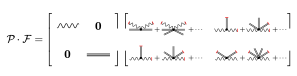
\includegraphics[width=1\textwidth]{./figures/drawing.png}
    \caption*{}
\end{figure}
Where a red line at the end of a vertex leg denotes the functional derivative with respect to the corresponding field.
To extract the gauge field anomalous dimension from the FRGE, we act on it with
a projection operator $\varPi_A$, which then annihilate all terms which does not originate from the diagrams with two external photon legs.
The only vertices that may form such diagrams come from terms of the form $\delta_{A}\delta_h \int c \cdot AAh$ and $\delta_h \delta_h \int c \cdot AAhh$
a projection operator $\varPi_A$, which then annihilate all terms which does not originate from the diagrams with two external photon legs.
The only vertices that may form such diagrams come from terms of the form $\delta_{A}\delta_h \int c \cdot AAh$ and $\delta_h \delta_h \int c \cdot AAhh$
\begin{figure}[H]
    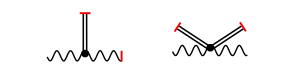
\includegraphics[width=1\textwidth]{./figures/vertices.png}
    \caption{Necessary vertices for computing gauge field anomalous dimension. Red line at the end of a vertex leg denotes a functional derivative with respect to the corresponding field applied to the interaction term}
\end{figure}
We denote the expressions for these vertices, respectively
\begin{gather}
    \left. \frac{\delta^2 \Gamma}{\delta h^{\mu\nu}(p_1) \delta A^{\rho}(p_2)}\right|_{h=0} = \frac{\delta^2}{\delta h^{\mu\nu}(p_1) \delta A^{\rho}(p_2)} \int \prod_{i=1}^3 d^4 p_i \mathcal{L}_{\text{AAh}}\left(\tilde{h}(p_1), \tilde{A}(p_2), \tilde{A}(p_3)\right)\\
    \left. \frac{\delta^2 \Gamma}{\delta h^{\mu\nu}(p_1) \delta A^{\rho}(p_2)}\right|_{h=0} = \frac{\delta^2}{\delta h^{\mu\nu}(p_1) \delta A^{\rho}(p_2)} \int \prod_{i=1}^3 d^4 p_i \mathcal{L}_{\text{AAh}}\left(\tilde{h}(p_1), \tilde{A}(p_2), \tilde{A}(p_3)\right)\\
    = \operatorname{VertAAh}_{\mu\nu\rho}(p_1,p_2,p_3)\\
    \left. \frac{\delta^2 \Gamma}{\delta h^{\mu\nu}(p_1) \delta h^{\rho\sigma}(p_2)}\right|_{h=0} = \frac{\delta^2}{\delta h^{\mu\nu}(p_1) \delta h^{\rho\sigma}(p_2)} \int \prod_{i=1}^4 d^4 p_i \mathcal{L}_{\text{AAhh}}\left(\tilde{h}(p_1), \tilde{h}(p_2), \tilde{A}(p_3), \tilde{A}(p_4) \right)\\
    \left. \frac{\delta^2 \Gamma}{\delta h^{\mu\nu}(p_1) \delta h^{\rho\sigma}(p_2)}\right|_{h=0} = \frac{\delta^2}{\delta h^{\mu\nu}(p_1) \delta h^{\rho\sigma}(p_2)} \int \prod_{i=1}^4 d^4 p_i \mathcal{L}_{\text{AAhh}}\left(\tilde{h}(p_1), \tilde{h}(p_2), \tilde{A}(p_3), \tilde{A}(p_4) \right)\\
     = \operatorname{VertAAhh}_{\mu\nu\rho\sigma}(p_1,p_2,p_3,p_4)
\end{gather}
Where $\mathcal{L}_{\text{AAh}}$, $\mathcal{L}_{\text{AAhh}}$ is the sum of terms from lagrangian proportional to the suitable power of fields.
\textcolor{red}{(expr. for vertices or ref. to apx)}
 
\subsubsection{Calculation of feynman \jhkbf{These are not feynman ...} diagrams}
Where $\mathcal{L}_{\text{AAh}}$, $\mathcal{L}_{\text{AAhh}}$ is the sum of terms from lagrangian proportional to the suitable power of fields.
\textcolor{red}{(expr. for vertices or ref. to apx)}
 
\subsubsection{Calculation of feynman \jhkbf{These are not feynman ...} diagrams}
\textcolor{red}{(...)} Then, continuing the argument from previous section, the contribution from second term that will not be annihilated
by $\varPi_A$ comes from products of effective vertices and propagators that involve only the second power of gauge field.
There are just two such products. After considering coefficients in the expansion of logarithm from (\ref{pf}) and from performing trace, the expression for gauge field renormalization beta function can be written as
\begin{align}
    \beta_{Z_A} & = \varPi_A \cdot \partial_t \Gamma_k = \varPi_A \left( \frac{1}{2} \widetilde{\partial_t} \int d^4 q \ \operatorname{VertAAhh}_{\mu\nu\rho\sigma}(p,-p,q,-q) \operatorname{PropG}^{\mu\nu\rho\sigma}(q)\right.\\
    & - \frac{1}{2} \widetilde{\partial_t} \int d^4 q \ \operatorname{VertAAh}^{\mu\nu\rho}(p,-q,p+q) \operatorname{VertAAh}^{\sigma\tau\kappa}(-p,q,-p-q) \cdot \\
    &\left. \cdot \operatorname{PropG}_{\mu\nu\sigma\tau}(p+q) \operatorname{PropA}_{\rho\kappa}(q) \phantom{\frac{}{}} \hspace{-0.35em}\right)
\end{align}
This reduces the problem of extracting information about RG flow in functional renormalization group to computing amputated one-loop feynman diagrams.
\begin{figure}[H]
    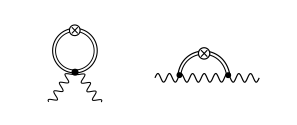
\includegraphics[width=1\textwidth]{./figures/diags.png}
    \caption{Feynman diagrams contributing to the anomalous dimension of gauge field. Wavy line denotes a photon propagator
    and the double straight line denotes the graviton propagator. A crossed circle denotes an insertion of the regulator.}
    \label{diags}
\end{figure} 

\textcolor{red}{(...)}\\

Finally, the resulting beta function of abelian gauge coupling $g$ in the spacetime with four dimensions is
\begin{equation}
    \beta_{g_1} = g_1 \frac{\eta_A}{2} = g_1 \frac{G}{4 \pi} \left( \frac{6 - \eta_h}{6(1-2 \Lambda)^2} + 
    \frac{(\eta_A-8)(1-2\Lambda) + (\eta_h -8)}{8 (1-2 \Lambda )^2}\right) + \beta_{g_1}^{\text{SM}}
    \beta_{g_1} = g_1 \frac{\eta_A}{2} = g_1 \frac{G}{4 \pi} \left( \frac{6 - \eta_h}{6(1-2 \Lambda)^2} + 
    \frac{(\eta_A-8)(1-2\Lambda) + (\eta_h -8)}{8 (1-2 \Lambda )^2}\right) + \beta_{g_1}^{\text{SM}}
\end{equation}
The result for an arbitrary spacetime dimension is given in (apx).
To study the qualitative aspects of gravitational corrections, we can neglect the cosmological constant and
the corrections to gauge and graviton propagators entering via $\eta_A$ and $\eta_h$. This approximations
yields a very simple form of beta function, that indicates a negative gravitational contribution to the running
of gauge coupling.
\begin{equation}
    \beta_{g_1} = - \frac{G}{4 \pi} + \beta_{g_1}^{\text{SM}}
    \beta_{g_1} = - \frac{G}{4 \pi} + \beta_{g_1}^{\text{SM}}
\end{equation}

\textcolor{red}{(...)}\\

Beta functions extracted from the full EA cannot depend on the choice of gauge parameters.
Introducing truncations, however, means that gauge dependence may not cancel entirely.
%% ?? Że będziemy sprawdzać zależność od gauge parameter ?? - tylko od beta w gravity gauge fixing (z jakiegoś powodu) - na alfy możemy też zrobić rg flow i one jakoś dążą do zera i jest argument że są nieważne (poczytać)
Another in principle redundant choice is a form of the regulator. For two different regulators,
$\Gamma_k$ will include field modes weighted in a different manner, so this choice simply
sets the definition of the object $\Gamma_k$. 
This means, that beta functions computed with different regulators will differ, but
if the regulator is picked in such way that it executes a proper IR cutoff,
it will always give the same results in the physical limit $k \rightarrow 0$. There should be no
qualitative differences in the behaviour of RG flow computed with different regulators.
%% Coś o tym że to będziemy tu sprawdzać
\jhkbf{Zrobić obliczenia dla różnych $\beta_h$ (to już de facto masz) i różnych regulatorów i przedyskutować wyniki.\\ 
W summary albo future directions możesz omówić wyniki które ja otrzymałem z astrid
}
\jhkbf{Zrobić obliczenia dla różnych $\beta_h$ (to już de facto masz) i różnych regulatorów i przedyskutować wyniki.\\ 
W summary albo future directions możesz omówić wyniki które ja otrzymałem z astrid
}
\textcolor{red}{
CO JEST JESZCZE DO ZROBIENIA\\
Cytowania w rozdziale 1\\
Background field i techniczne sprawy w rozdziale 2\\
Summary dyskusji wyników z asymptotic safety, powiedzieć o predictivity np weak gravity bound i higgs mass\\
Ogarnąć przestrzeń pędową, całki i pochodne funkcyjne jak to działa od A do Z\\
Jak wchodzi gauge fixing i dlaczego pomijamy duchy\\
Sekcja 3.1.2\\
Prezentacja i dyskusja wyników\\
Systematycznie wypisać wszystkie wykorzystywane przybliżenia i przedyskutować ich wpływ, ważność i możliwą weryfikację czy działają\\
Introduction i summary
}


\section*{Summary}

\begin{thebibliography}{9}
    \bibitem{pdg}
    Workman, R.L. et al. (Particle Data Group), Prog. Theor. Exp. Phys. 2022, 083C01 (2022) and 2023 update
    \bibitem{book}
    Hamber, H. W. (2009). Quantum Gravitation – The Feynman Path Integral Approach. Springer Nature. ISBN 978-3-540-85292-6.
    \bibitem{wetteq}
    Wetterich, C. (1993). Exact evolution equation for the effective potential. Physics Letters B, 301(1). https://doi.org/10.1016/0370-2693(93)90726-x 
    \bibitem{higgs mass}
    Shaposhnikov, M., Wetterich, C. (2010). Asymptotic safety of gravity and the Higgs boson mass. Physics Letters B, 683(2-3). https://doi.org/10.1016/j.physletb.2009.12.02    
    \bibitem{wilczek}
    Robinson, S., Wilczek, F. (2006). Gravitational Correction to Running of Gauge Couplings. Phys. Rev. Lett., 96(23). https://doi.org/10.1103/PhysRevLett.96.231601
    \bibitem{pietrykowski}
    Pietrykowski, A. (2006). Gauge Dependence of Gravitational Correction to Running of Gauge Couplings. Phys. Rev. Lett., 98(6). https://doi.org/10.1103/physrevlett.98.061801
    \bibitem{toms}
    Toms, D. J. (2007). Quantum gravity and charge renormalization. Physical Review D, 76 (4). https://doi.org/10.1103/physrevd.76.045015
    \bibitem{absence}
    Ebert, D., Plefka, J., Rodigast, A. (2008). Absence of gravitational contributions to the running Yang–Mills coupling. Physics Letters B, 660(5). https://doi.org/10.1016/j.physletb.2008.01.037 
    \bibitem{tang}
    Tang, Y., Wu, Y.-L. (2010). Gravitational Contributions to Running of Gauge Couplings. Communications in Theoretical Physics, 54(6). https://doi.org/10.1088/0253-6102/54/6/15
    \bibitem{nieuwenhuizen}
    Deser, S., van Nieuwenhuizen, P. (1974). Nonrenormalizability of the Quantized Einstein-Maxwell System. Physical Review Letters, 32(5). https://doi.org/10.1103/physrevlett.32.245
    \bibitem{qeg}
    Reuter, M., Saueressig, F. (2012). Quantum Einstein gravity. New Journal of Physics, 14 (5). https://doi.org/10.1088/1367-2630/14/5/055022
    \bibitem{reuter_abelian}
    Daum, J.-E., Harst, U., Reuter, M. (2010) Running gauge coupling in asymptotically safe quantum gravity. J. High Energ. Phys., 84(2010). https://doi.org/10.1007/JHEP01(2010)084
    \bibitem{christiansen_eichhorn}
    Christiansen, N., Eichhorn, A. (2017). An asymptotically safe solution to the U(1) triviality problem. Physics Letters B, 770. https://doi.org/10.1016/j.physletb.2017.04.047
    \bibitem{kwapisz_eichhorn}
    Eichhorn, A., Kwapisz, J.H., Schiffer, M. (2022). Weak-gravity bound in asymptotically safe gravity-gauge systems. Phys. Rev. D, 105(10). https://doi.org/10.1103/PhysRevD.105.106022
\end{thebibliography}

\end{document}